\documentclass[11pt,toc=sectionentrywithoutdots, 
headheight=44pt, headings=optiontoheadandtoc, hyperfootnotes=false, hypertexnames=false]{scrartcl}

%Packages
\usepackage{geometry}

\geometry{
a4paper, 
left=30mm, 
right=25mm, 
top=25mm, 
bottom=25mm, 
headsep=5mm, 
footnotesep=5mm,
headheight=20mm,
footskip=15mm,
marginparwidth=15mm
}

\usepackage[utf8]{inputenc}
\usepackage{csquotes}
\usepackage{times}
\usepackage{verbatim}
\usepackage[T1]{fontenc}
\usepackage[ngerman]{babel}
\usepackage{graphicx}
\usepackage[headsepline]{scrlayer-scrpage}
\usepackage{blindtext}
\usepackage{footnotebackref}
\usepackage{nameref}
\usepackage{setspace}
\usepackage[automake]{glossaries}
\usepackage[export]{adjustbox}
\usepackage{wrapfig,lipsum,booktabs}
\usepackage{placeins}
%\captionsetup[wraptable]{margin=x cm, width= y cm}
\usepackage{caption}
\usepackage{mathtools}
\usepackage{eurosym}

\newcommand\extendedref[1]{Siehe \ref{#1}}
\newcommand\fullref[1]{\extendedref{#1} auf Seite \pageref{#1}}



\setstretch{1.2}

\usepackage[
backend=biber,
style=authortitle,
citestyle=authoryear
]{biblatex}

\addbibresource{literatur.bib}

 \usepackage{tikz,ifthen,xstring,calc,pgfkeys,pgfopts}
 \usepackage{tikz-uml}
 %\usetikzlibrary{external}
 %\tikzexternalize[prefix=figures/] % activate and define figures/ as cache folder

\usepackage{hyperref}
\usepackage[printonlyused, withpage]{acronym}

%%%%%%%%%%%%%%%%%% Compile optimization - Kill for release!!!%%%%%%%%%%%%%%
% Kill draft in Dokumentclass!!!
%\pdfcompresslevel=0
%\pdfobjcompresslevel=0
%%%%%%%%%%%%%%%%%%%%%%%%%%%%%%%%%%%%%%%%%%%%%%%%%%%%%%%%%%%%%%%%%%%%%%%%

\hypersetup{
    colorlinks=true,
    linktoc=page,
    linkcolor=blue,
    filecolor=magenta,      
    urlcolor=blue,
    citecolor=blue
}



%%%%%%%%%%%%%% Set line Spacing for Abbreviation %%%%%%%%%%%%%%%%%%
%\renewenvironment{description}
%{\list{}{\labelwidth0pt\itemindent-\leftmargin
%    \parsep0pt\itemsep0pt\let\makelabel\descriptionlabel}}
%               {\endlist}
%%%%%%%%%%%%%%%%%%%%%%%%%%%%%%%%%%%%%%%%%%%%%%%%%%%%%%%%%%%%%%%%%%%%%%

%\usetikzlibrary{external}
%\tikzexternalize %

%Function for getting sectionName---------------------------------------------------

\newcounter{secautolabel}
\AddtoDoHook{heading/endgroup}{\setautolabel}
\newcommand*{\setautolabel}[1]{%
  \stepcounter{secautolabel}%
  \label{sec:autolabel:\thesecautolabel}%
  \expandafter\xdef\csname #1title\endcsname{%
    \noexpand\nameref*{sec:autolabel:\thesecautolabel}%
  }%
}

\newcommand\sectionRefs{%
	\sectiontitle  
}


%Function for getting sectionName----------------------------------------------------



%Images path
\graphicspath{{./src/images/}}

%Document meta data
\geometry{bottom=25mm, right=25mm, left=25mm, top=35mm}

%Set page numbering font
\renewcommand{\headfont}{\normalfont}

\makeglossaries

\newglossaryentry{Query}
{
	name=Query,
	description={Datenbankanweisung, welche an einen Datenbankserver 		verschickt wird und dazu dient, Daten abzufragen, zu erstellen, zu verändern oder zu löschen}
}
\newglossaryentry{Assembly}
{
	name=Assembly,
	description={Logische Organisationseinheit in .NET, welche einen Baustein einer größeren Anwendung darstellt. Auch \glqq Komponente\grqq{} oder \glqq Modul\grqq{} genannt}
}
\newglossaryentry{Persistenz}
{
	name=Persistenz,
	description={Die theoretische Möglichkeit eines Objekts unendlich und unabhängig von der Software, in der es erzeugt wurde, zu existieren. In der Praxis kann keine hundertprozentige Persistenz gewährleistet werden}
}
\newglossaryentry{Customer Obsession}
{
	name=Customer Obsession,
	description={Wirtschaftsphilosophie, die den Kunden als Maßstab für alle Überlegungen des ökonomischen Denken und Handels emporhebt. Gemäß dieses Ansatzes gibt es keine den Wünschen des Kunden übergeordneten Maxime}
}
\newglossaryentry{Kanban}
{
	name=Kanban,
	description={Prinzip für das Abarbeiten von Aufgaben im Team, bei dem alle anfallenden Aufgaben mit einer Karte visualisiert werden, die in Säulen von festgelegter maximaler Stückzahl abgelegt sind. Steigt eine Aufgabe im Bearbeitungsstadium auf, wird sie von links nach rechts \glqq gepullt\grqq{}. Die rechteste Säule trägt immer den Namen \glqq Done\grqq}
}
\newglossaryentry{Product Owner}
{
	name=Product Owner,
	description={\glqq Der:die Product Owner:in ist ergebnisverantwortlich für die Maximierung des Wertes des Produkts, der
sich aus der Arbeit des Scrum Teams ergibt. Wie dies geschieht, kann je nach Organisation, Scrum Team
und Individuum sehr unterschiedlich sein\grqq\footnote{Entnommen aus \cite{SchwaberSutherland2020}}}
}
\newglossaryentry{Pain Driven Development}
{
	name=Pain Driven Development,
	description={\glqq Pain Driven Development, or PDD, is the practice of writing software in such a way that you only \glq fix\grq{} problems when they are causing pain, rather than trying to preempt every possible issue\grqq\footnote{Entnommen aus \cite{Smith2017}}}
}
\newglossaryentry{Refaktorierung}
{
	name=Refaktorierung,
	description={\glqq Code-Refactoring ist der Prozess der Umstrukturierung bestehenden Quellcodes ohne dessen externes Verhalten zu ändern. Refactoring verbessert keine funktionalen Attribute der Software. Die Vorteile von Refactoring umfassen verbesserte Lesbarkeit des Codes und reduzierte Komplexität\grqq\footnote{Entnommen aus \cite{Kranz2021}}}
}
\newglossaryentry{IntelliSense}
{
	name=IntelliSense,
	description={Von Microsoft entwickeltes Werkzeug für die integrierten Entwicklungsumgebungen Visual Studio und Visual Studio Code, welches der Programmiererin während beim Entwickeln eine Übersicht darüber gibt, welche Variablen, Klassen und Methoden an der gerade zu bearbeiteten Stelle im Code zur Verfügung stehen}
}
\newglossaryentry{Legacy Code}
{
	name=Legacy Code,
	description={Code, der von mittlerweile nicht mehr kontaktierbaren Entwicklern \glqq geerbt\grqq wurde, nicht mehr in allen Aspekten dem aktuellen Stand der Technik entspricht und darüber hinaus nicht umfassend dokumentiert ist}
}
\newglossaryentry{Open Source}
{
	name=Open Source,
	description={Software, die von den Entwickler öffentlich zur Verfügung gestellt wird, ohne dass dabei Kosten für Interessenten anfallen. Die entsprechende Software kann für jeden erdenklichen Zweck verwendet, also auch erweitert oder modifiziert werden. Ebenso kann Open-Source-Software für kommerzielle Zwecke verwendet werden}
}
\newglossaryentry{Breakpoint}
{
	name=Breakpoint,
	description={Markierung am Rand der Zeile im Programmcode, an der die Ausführung des Programms an eben dieser Stelle angehalten wird. Nach dem Anhalten kann im Code-Editor bzw. der integrierten Entwicklungsumgebung der aktuelle Status von Variablen abgefragt werden und bei Bedarf Zeile für Zeile weiter ausgeführt werden}
}
\newglossaryentry{Single Responsibility Principle}
{
	name=Single Responsibility Principle,
	description={Das erste Prinzip aus den fünf vom Softwareentwickler Robert C. Martin formulierten \glq SOLID\grq{}-Prinzipien, welches besagt, das ein Modul nur einen einzigen Grund haben sollte, sich zu ändern. Beispielsweise kann sich ein Modul entweder in Hinblick auf die GUI ändern oder in Hinblick auf die Datenbankkommunikation, aber niemals mal das eine, mal das andere}
}
\newglossaryentry{Abstrakte Klasse}
{
	name=Abstrakte Klasse,
	description={Klasse aus der kein Objekt instanziert werden kann. Abstrakte Klassen dienen als Blaupause für weitere Klassen, welche von ihr erben}
}
\newglossaryentry{SqlCommand}
{
	name=SqlCommand,
	description={Nicht mit \glqq Query\grqq{} zu verwechseln. Es handelt sich um eine Klasse aus .NET. Diese speichert Parameter, die für Tabellenspalten stehen, die dazugehörigen Datentypen und eine schematische Query mit Platzhaltern für Werte, die in den Spalten gespeichert werden sollen}
}
\newglossaryentry{Boolean}
{
	name=Boolean,
	description={Standard-Datentyp aus allen bekannten Programmiersprachen, der entweder den Wert \glqq wahr\grqq{} oder \glqq falsch\grqq{} annehmen kann}
}
\newglossaryentry{Datenbank Management System}
{
	name=Datenbank Management System,
	description={Komplexe Applikation mit ausführlicher graphischer Benutzeroberfläche, das für die Arbeit mit Datenbanken und Datenbankanfragen konzipiert ist. Obwohl diese Programme keine Voraussetzung dafür sind, mit Datenbanken zu arbeiten (denn erfahrene Informatikerinnen können dies auch manuell), arbeitet nahezu jedes Unternehmen mit einem solchen System}
}



 
\begin{document}
\pagenumbering{Roman}
\thispagestyle{empty}

\cfoot[]{}
%\ofoot{Seite \thepage\:von \pageref{LastPage}}
\ofoot{\thepage}
\ifoot{© Frank Loleit}
\ohead{
\includegraphics[scale=0.125]{argusLogo}}



\ihead
{%	
	\begin{small}
	
	
		MODUL FÜR GEKAPSELTE DATENBANKKOMMUNIKATION%		
		\newline\
		\textit\sectionRefs
	\end{small}%
}
%IHK-Logo
\begin{figure}[h]

\includegraphics[scale=0.25]{ihkLogo}
\centering
\end{figure}
\begin{center}
\begin{Large}

Abschlussprüfung Winter 2021
\linebreak

Fachinformatiker (Anwendungsentwicklung)\linebreak
Dokumentation der betrieblichen Projektarbeit
\linebreak\linebreak
\end{Large}


\begin{LARGE}
\begin{bfseries}
	Entwicklung eines Moduls in einer Desktopanwendung zur Umstellung von direkten Datenbankzugriffen zu einer gekapselten Datenbankkommunikation mit optionaler Simulationsmöglichkeit.
\linebreak\linebreak
\end{bfseries}
\end{LARGE}

\begin{Large}
%Backend-Applikation zur algorithmusbasierten 
%Erfassung von\linebreak Meldungen in sozialen Netzwerken
%\linebreak

Abgabetermin: 22.11.2021
\linebreak\linebreak
\begin{bfseries}
Auszubildender:\linebreak
\end{bfseries}
Frank Loleit\linebreak
Wildenbruchstr. 43\linebreak
12435 Berlin\linebreak

\begin{figure}[h]

\includegraphics[scale=0.25]{argusLogo}
\centering
\end{figure}



\begin{bfseries}
Ausbildungsbetrieb:\linebreak
\end{bfseries}
ARGUS DATA INSIGHTS® Deutschland GmbH\linebreak
Gneisenaustr. 66\linebreak
10961 Berlin


\end{Large}


\end{center}
\newpage
\setcounter{page}{1}
\pagenumbering{Roman}


\tableofcontents


\setcounter{secnumdepth}{0}

\newpage

\phantomsection
\addcontentsline{toc}{section}{Abbildungsverzeichnis}
\listoffigures




%\newpage

\phantomsection
\addcontentsline{toc}{section}{Tabellenverzeichnis}
\listoftables
%\newpage

%\section{Listings}
%\blindtext\blindtext\blindtext
%\newpage

\section{Abkürzungsverzeichnis}


\begin{acronym}[xxxxxxx]

\acro{ADI}{Argus Data Insights Deutschland GmbH}
\acro{CRUD}{Create, Read, Update, Delete}
\acro{GUI}{Graphical User Interface}
\acro{XAML}{Extensible Application Markup Language}
\acro{DRY}{Don't Repeat Yourself}
\acro{SQL} {Structured Query Language}
\acro{SSMS} {SQL Server Management Studio}
\acro{PO} {Product Owner}

\end{acronym}
%\newpage

\phantomsection
\addcontentsline{toc}{section}{Glossar}
\printglossary[nonumberlist]
\newpage


\setcounter{secnumdepth}{1}
\pagenumbering{arabic}
\setcounter{secnumdepth}{4}
\ofoot{Seite\:\thepage}%\:von \pageref*{myLastPage}%}

\section{Einleitung}
In diesem Projekt wird das Ziel verfolgt, die Datenbankkommunikation einer Desktopanwendung zu vereinheitlichen und die Arbeit der Entwickler von der Arbeit der Nutzer abzugrenzen. Obgleich es sich bei dem entwickelten Modul um ein Werkzeug handelt, das nur von Entwicklern geöffnet und verwendet werden kann, steht der Kunde im Vordergrund aller Bemühungen. Denn sowohl das Auffinden und Lösen von Programmfehlern, wie auch das Implementieren von neuen Komponenten kann durch die Vereinheitlichung und Separierung der Datenbankoperationen deutlich effizienter werden. Der Kunde erhält dadurch nicht nur ein tendenziell stabileres System, sondern kann auch damit rechnen, dass neue gewünschte Funktionalitäten schneller umgesetzt werden. In diesem Sinne steht bei allen Bemühumgen dieses Projektes stets die \gls{Customer Obsession} im Vordergrund.

\subsection{Projektbeschreibung}
Ausgangspunkt der Arbeit ist die Desktopapplikation \glqq Arche\grqq{}, entwickelt im .NET-Framework\footnote{\cite{Microsoft2020}} 3.5 mit WinForms-\acs{GUI}. Das Debugging gestaltet sich teils als recht aufwändig, da alle Funktionen umgangen werden müssen, die Kundendaten generieren, verändern oder löschen. Grund dafür ist das Fehlen von Mechanismen, durch die sich Datenbankoperationen, die von Kunden und Entwicklern vorgenommen werden, jeweils voneinander abgrenzen lassen. Auch das Implementieren von neuen datenbanksensiblen Features gestaltet sich als umständlich, da es kein einheitliches Prinzip für die Datenbankkommunikation gibt. Viel mehr hat jeder einzelne Workflow jeweils eine eigene Klasse für die Datenbankkommunikation, die sich inhaltlich aber kaum unterscheiden, sondern im Wesentlichen voneinander kopiert wurden und das \acs{DRY}-Prinzip wenig Berücksichtigung findet. Daher soll ein Modul entwickelt werden, dass die Kommunikation mit der Datenbank kapselt.\newline\newline Zunächst soll es möglich sein, dass eine \gls{Query}, die ein beliebiger Workflow an den Datenbankserver übergibt, zurückgehalten werden kann und somit nicht Gefahr zu laufen, unerwünschte Änderungen an Datenbankeinträgen vorzunehmen. Dabei soll in einer für Entwickler bestimmten GUI die entsprechende Query mit sinnvoller Hervorhebung entsprechender Keywords erfolgen. Zudem soll der Entwickler frei entscheiden können, ob die Query verarbeitet, zurückgehalten oder in ein \acs{SQL}-Management-System übertragen werden soll. Im Anschluss soll die uneinheitliche Datenbankkommuniktation durch eine globale Logik mit Hilfe von Datenbankmodellen ersetzt werden. Aus diesen Modellen soll schlussendlich ein einheitliches Verfahren abgeleitet werden können, das die Datenbankanbindung auf ein einziges \gls{Assembly} des Projektes konzentriert und somit eine langfristige Arbeitserleichterung schafft.

\subsection{Projektziel}
Nach Abschluss des Projektes muss es möglich sein, in Arche Insert-, Update- und Delete-Funktionen auszulösen, ohne dabei Kundendaten zu beeinträchtigen. Ist das zu entwickelnde Modul aktiv und es wird in der GUI von Arche ein Speichern- oder Löschen-Button geklickt, soll Arche angehalten und stattdessen ein Fenster öffnen, das nur für Entwickler bestimmt ist. Dieses gibt nun die Query aus, welche an den Datenbankserver geschickt worden wäre. Die Möglichkeit, die Query mit einem Klick umgehend nach \acs{SSMS} zu versenden muss ebenfalls gegeben sein, wie die Funktion, frei entscheiden zu können, ob die Query von Arche ausgeführt wird oder nicht. Die Entwickler müssen die Möglichkeit erhalten die Datenbank lokal zu simulieren und die entsprechenden Queries lokal auszuführen. Zudem muss ein einheitliches auf Datenbankmodellen basierendes Prinzip implementiert werden, über welches jedwede Insert-, Update- und Delete-Query mit entsprechenden Parametern generiert werden kann.%keine Unstimmigkeiten mit dem 
%Webinterface auftreten. Die \acs{ADI} ist daher bemüht weitere Schritte %einzuleiten. Man hat sich entschieden \acs{XAML} zu verwenden. Auch %Mathematisch ist dies wichtig\footnote{vgl. \cite{GeraldTeschl2008}}.

\subsection{Projektumfeld}
Argus Data Insights (im Folgenden \glqq Argus\grqq{} genannt) ist darauf spezialisiert, Print- , Video- und Onlinemedien - insbesondere Zeitungen, Fernsehen und soziale Netzwerke - für angefragte Zeiträume und Themen zu durchsuchen und dem Kunden skalierbare Dossiers mit Informationen zur eigenen Person, Firma oder Einrichtung zu geben. Die Kunden erlangen auf diese Weise einen detaillierten Einblick darüber, wie viel Aufmerksamkeit der Kunde in den Medien allgemein erhält, welche Themen mit dem Kunden assoziiert werden und und die Berichterstattung tendenziell positiv, negativ oder neutral ausfällt. Die Redaktionssoftware Arche wird sowohl zum Digitalisieren, Annotieren, Aufbereiten und Versenden der für den Kunden angefertigten Dossiers verwendet. Dabei werden vor allem Print- und Onlineinhalte unterschieden. Die verschiedenen Medieninhalte werden in Fileservern abgelegt, deren Pfade sowie zahlreiche Medienparameter in Datenbanktabellen gespeichert. Darüber hinaus gibt es eine umfangreiche Kundendatenbank. Datenbankzugriffe erfolgen nicht einheitlich, sondern von verschiedenen \gls{Persistenz}-Klassen aus, deren interne Logik von jeweils der zuletzt angelegten Persistenzklasse kopiert ist (nicht vererbt).

\subsection{Projektbegründung}
Die Gründe für das Projekt liegen in der erschwerten Wartung der Software, sowie dem erhöhten Aufwand, neue datenbanksensible Komponenten hinzuzufügen. Muss ein Ticket\footnote{Bei Argus wird das \gls{Kanban}-Board \href{https://www.atlassian.com/software/jira}{Atlassian Jira} verwendet.} bearbeitet werden, bei dem ein Problem mit Query und/oder Datenbank vermutet wird, müssen beim Debugging sehr früh Breakpoints gesetzt werden, um nicht Gefahr zu laufen, Kundendaten irreversibel zu verändern. Es fehlt die Möglichkeit, global die Ausführung von Datenbankprozessen zurückzuhalten. Darüber hinaus ist es äußerst kompliziert, die entsprechende Query zu erhalten, welche es für das jeweilige Ticket zu analysieren gilt. Daran anschließend ist kein einheitlicher Prozess vorhanden, der die Kommunikation von .NET und MSSQL steuert. Um sowohl Wartbarkeit, als auch einfache Erweiterbarkeit zu gewährleisten, ist dieses Projekt in Absprache mit den \gls{Product Owner}n entstanden.

\subsection{Projektabgrenzung}
Was die technische Abgrenzung anbelangt, ist durch die komponentenorientierte Arbeitsweise in .NET das zu entwickelnde Modul gut von bereits fertigen Projekten innerhalb der Kernapplikation getrennt. Konkret bedeutet das, dass das neue Modul \glqq DBEncapsulation\grqq{} und dessen Testmodul \glqq DBEncapsulationTests\grqq{}\footnote{\extendedref{fig:Assemblies}} per se isoliert und interagieren nur dann mit der Hauptapplikation Arche, wenn eine Referenz zu einem anderen Modul hergestellt wird. Wird eine Variable oder Methode aus DBEncapsulation als öffentlich deklariert, ist sie dennoch vorerst in keinem der anderen Module verfügbar und trägt nicht zur Überlastung der \gls{IntelliSense} bei. Soll das Modul aus einem bereits entwickelten Modul verfügbar sein, muss dessen Projektdatei zunächst eine Referenz auf DBEncapsulation hinzugefügt werden. Im nächsten Schritt kann denjenigen Klassen, welche datenbankrelevante Prozesse implementieren ein \glqq using\grqq{}-Statement hinzugefügt werden. Erst unter diesen Voraussetzungen, sind in der entsprechenden Klasse Daten verfügbar, die als öffentlich deklariert sind.\newline\newline Bezüglich der inhaltlichen Abgrenzung ist festzuhalten, dass aufgrund der hohen Vielfalt an Datenbankoperationen zunächst Insert- Update- und Delete im Vordergrund stehen werden. Da Select-Operationen keine Beeinträchtigungen von Kundendaten zur Folge haben können, wird für diese Fälle vor allem im Vordergrund steht den Entwicklern ein korrektes Feedback darüber zu geben, welche Tabellen und Spalten nach welcher Abfragelogik an die Datenbank übermittelt wurden. Da Select-Operationen stark heterogen sind, wird hier kein einheitlicher Prozess für angestrebt. Jedoch soll es für die Fälle Update, Insert und Delete grundsätzlich nicht mehr nötig sein, neue Logiken für neue Module zu entwerfen und lediglich durch Referenzierung auf DBEncapsulation entsprechende Funktionalitäten bereit gestellt werden.

\section{Projektplanung}
Für die Planung ist wesentlich, dass das Tagesgeschäft der Entwicklerinnen bei Argus nicht unterbrochen wird, sondern parallel zum hier dokumentierten Projekt mit allen zeitlichen und finanziellen Aufwendungen weiterläuft. Das heißt, bei der Projektplanung ist ein sinnvolles Verhältnis von Recherche, selbstständigem Kodieren und eigenverantwortlichen Entscheidungen einerseits, sowie zielgerichtete Unterstützung durch Ausbilder und Kolleginnen andererseits. Um den stetigen Austausch zu gewährleisten, wird der Fortschritt dieses Projektes im täglichen Meeting mit Vorgesetzten und Teammitgliedern geteilt. Zudem werden regelmäßige sowie spontane 1:1-Gespräche mit dem Ausbilder durchgeführt.

\subsection{Projektphasen}
Das Projekt wurde in einem Zeitraum von 70 Stunden umgesetzt. Dabei wurde die gesamte Stundenanzahl wie folgt aufgeteilt\footnote{\extendedref{sec:Detaillierte Zeitplanung}}:\newline

\begin{table}[ht]
	\begin{center}
		\begin{tabular}{ ||l|r|| }
			\hline
			\textbf{Projektphase} 		& \textbf{Geplante Zeit} \\
			\hline

			Analysephase 				& 7 h	 		\\
			Entwurfsphase				& 11 h	 		\\
			Implementierungsphase 		& 40 h	 		\\
			Abnahme und Einführung		& 2 h 			\\
			Erstellen der Dokumentation & 10 h 			\\
			\hline
			\textbf{Gesamt}	 			& \textbf{70 h}	\\
			
			\hline
		\end{tabular}
		%\caption{Zeitplanung}
	\end{center}
\end{table}%
Den Einstieg in das Projekts betreffend ist zu erwähnen, dass es sich bei dem Projekt Arche um \gls{Legacy Code} handelt, dessen Funktionsweise nur begrenzt objektorientiert aufgebaut ist. Sowohl bei Analyse, Entwurf und Implementierung ist daher immer das Nachvollziehen des Codes durch Recherche, Debugging und Rücksprache mit erfahrenen Mitarbeitern entscheidend.

\subsection{Ressourcenplanung}
%Die notwendigen Ressourcen für das Projekt sind sowohl monetärer als auch nicht-monetärer Art. Nicht monetäre Ressourcen umfassen vor allem zeitliche Aufwendungen von Ausbilder und Kolleginnen, %sowie Recherche
Bei der Planung der Ressourcen\footnote{\extendedref{sec:Ressourcenplan}} kann zwischen Hardware- und Softwareressourcen unterschieden werden. Bei der Auswahl wurde darauf geachtet, keine neuen Kosten zu generieren. Bei der Hardware kamen daher die von Unternehmen und Bildungseinrichtung bereitgestellten Computer zum Einsatz. Die eingesetzte Software ist entweder \gls{Open Source} oder es existieren bereits entsprechende Lizenzen bei Argus. Das heißt, es wurden keine Ressourcen angeschafft, die vor Beginn des Projektes nicht vorhanden gewesen wären. Bezüglich des Personals ist ebenfalls festzuhalten, dass sowohl Ausbilder als auch Kolleginnen täglich kontaktierbar oder vor Ort waren. Code-Reviews und Einarbeitungen konnten in den Arbeitsalltag so integriert werden, dass keine neuen personellen Ressourcen notwendig wurden.

\subsection{Entwicklungsprozess}
Bevor der Entwicklungsprozess starten konnte, war es nötig, den Quellcode von Arche in ausgewählten Stellen zu debuggen. Dabei ging es nicht darum, Fehler zu beheben, sondern Schritt für Schritt den Code nachzuvollziehen. Dies war aus zweierlei Hinsicht sinnvoll: Zunächst hatte ich so die Möglichkeit, Wissen über C\# und die Arbeit mit Visual Studio zu sammeln und andererseits die zu bearbeitende Software Arche besser kennenzulernen. Hier wurde zunächst so vorgegangen, dass in der GUI von Arche der Text von Buttons und Labels in die Suchmaske des Visual-Studio-Explorers eingegeben wurden. Auf diese Weise konnten diejenigen Komponenten und Klassen identifiziert werden, welche für das Frontend an der entsprechenden Stelle genutzt wurden. Anschließend wurde weit oben im Code ein \gls{Breakpoint} gesetzt und dann im Debug-Modus einen Button aus der GUI geklickt.\newline\newline Da es bei diesem Projekt um Datenbankprozesse geht, wurden vor allem Buttons mit der Aufschrift \glqq Speichern\grqq{}, \glqq Aktualisieren\grqq{} oder \glqq Hinzufügen\grqq{} gewählt. Nun wurde in Absprache mit erfahrenen Kollegen der Code immer soweit weiter ausgeführt, bis die datenbankrelevante Funktion erreicht wurde, die Ausgangspunkt für dieses Projekt sein soll. Auf diese Weise konnte nicht nur die Funktionsweise von Arche besser verstanden, sondern auch jene Stellen bestimmt werden, an denen die hier zu entwickelnde Komponente andocken soll. An dieser Stelle muss erwähnt werden, dass es vor allem zu Beginn des Projektes nicht immer gelungen ist, Veränderungen an Datenbankeinträgen rechtzeitig zu unterbinden. Ungewollte Veränderungen von Daten kamen vor allem dadurch zustande, dass nicht immer klar war, ob eine Funktion die Beeinflussung von Daten vorbereitet oder bereits ausführt. Gelegentlich mussten daher einzelne Zeilen in der Datenbank manuell wieder eingefügt oder Rücksprache mit den Kunden gehalten werden. Diese Erfahrung war prägend für die generelle Herangehensweise an das Projekt, welche als \gls{Pain Driven Development} bezeichnet werden kann.

\section{Analysephase}
Hier macht es Sinn in eine technische, sowie eine wirtschaftliche Analyse einzuteilen. In technischer Hinsicht wurde bereits angemerkt, dass das Verständnis des Codes nicht über Dokumentationen, sondern über das Debugging und das Gespräch mit Kollegen funktioniert. Häufig viel dabei auf, dass Funktionen in Arche bei niedriger Schriftgröße deutlich über eine Bildschirmseite hinausreichen können und verschiedene Softwarebereiche wie die Logik der GUI nur schwach von der Datenverwaltung, zu der auch die Datenbanklogik gehört, getrennt wurden\footnote{\extendedref{fig:Vermischung verschiedener Aufgabenbereiche}}. Da auch generell wenig Signaturen und keine Kommentare im Code vorhanden sind, bestand die Aufgabe darin, zunächst zu mutmaßen, welche Teile des Codes mit dem Speichern von Daten zusammenhängen könnten und welche jedwede anderen Funktionen erfüllen, die mit diesem Projekt nicht zusammenhängen.\newline Was die wirtschaftliche Analyse betrifft, ist nicht zuletzt der Zeitaufwand zu beachten, der notwendig wird, wenn wie im vorliegenden Fall das \gls{Single Responsibility Principle} nicht eingehalten wird.

\subsection{IST-Zustand}
Die Datenbankkommunikation von Arche ist so organisiert, dass verschiedene Medienklassen (z.B. Printmedien, Onlinemedien, Socialmedia-Posts usw.) jeweils eine Persistence-Klasse zur Verfügung haben. Benannt sind diese ungefähr nach Mediumname, z.B. \glqq PrintmedienTreffer.cs\grqq{} und \glqq PrintmedienTrefferPersistence.cs\grqq{}. Erstere enthält diverse Variablen und Funktionen, die mit dem entsprechenden Medium zusammenhängen\footnote{\extendedref{fig:PrintmedienTreffer.cs}}. Es gibt zwar auch hier keine Dokumentation, jedoch finden sich hier und da Kommentare der Entwicklerinnen, die Aufschluss über die entsprechende Geschäftslogik geben können. Es muss jedoch davon ausgegangen werden, dann nicht alle Variablen noch immer benötigt werden und womöglich datenbankrelevante und nicht datenbankrelevante Variablen vermischt sind. Die \gls{Abstrakte Klasse} \glqq AbstractTreffer\grqq{}\footnote{\extendedref{fig:AbstractTreffer.cs}} wiederum bildet die Basis für alle Medienklassen und enthält verschiedene Parameter, wie z.B mehrere Identifikationsnummern.\newline Was die boolischen Werte anbelangt, ist zum Verständnis zu erwähnen, dass in Arche Benennungen wir \glqq deleted\grqq{} oder \glqq loaded\grqq{} nicht den aktuellen Zustand eines Objektes beschreiben, sondern ausdrücken sollen, dass ein Objekt geladen oder gelöscht werden soll. Würde man also eine Neubenennung dieser boolischen Werte anstreben, wäre eine Formulierung wie \glqq toBeDeleted/toBeLoaded\grqq{} sinnvoll. Für das vorliegende Projekt steht jedoch zunächst die \gls{Refaktorierung} der Datenbanklogik, weniger der äußeren Form, im Vordergrund.\newline\newline Nutzt man in der Klasse \glqq AbstractTreffer\grqq{} die IntelliSense-Funktion für die Referenzabfrage der Funktion \glqq abstract int savePersistent()\grqq{}, werden 799 Implementierung in zahlreichen Klassen ausgegeben. Es ist also davon auszugehen, dass diese Funktion eine zentrale Rolle für das Ablegen von Daten in der Datenbank spielt. Ebenso wird hier der Arbeitsaufwand deutlich: Da die Funktion abstrakt ist, wird nur die Signatur übergeben. Für jede Klasse, die Daten mithilfe dieser Funktion abspeichern möchte, muss eine eigene Implementierung geschrieben werden. Dies ist zwar sicherlich dem Umstand geschuldet, für unterschiedliche Medien unterschiedliche Speichermechanismen zu benötigen, jedoch wird ist auch klar, dass Arbeitsaufwand zur Weiterentwicklung der Software unverhältnismäßig hoch ist. Obgleich Argus anstrebt, langfristig auf modernere Lösungen wie ASP.NET\footnote{\href{https://dotnet.microsoft.com/apps/aspnet}{https://dotnet.microsoft.com/apps/aspnet}} oder Angular\footnote{\href{https://angular.io/}{https://angular.io/}} zu setzen, ist das Unternehmen in der Situation, an jedem Wochentag Mediendossiers an Kunden ausliefern zu müssen. Der IST-Zustand der Entwicklung von datenbankrelevanten Komponenten kann also am treffendsten mit zu hoher finanzieller und zeitlicher Belastung beschrieben werden.

\subsection{Wirtschaftlichkeitsanalyse}
%Aus den obigen Erkenntnissen müssen nun also folgende Fragen abgeleitet werden: \textit{Wie lange dauert es durchschnittlich der Anwendung eine neue Persistence-Klasse hinzuzufügen? Wie viel %Kosten fallen bei der Entwicklung einer solchen Klasse an? Wie viel Zeit und Kosten können durch das Einführen einer gekapselten Datenbankkommunikation gespart werden?} Um dabei einen %realistischen Einblick in die Kostenstruktur geben zu können, ist
Um das vorliegende Projekt als wirtschaftlich betrachten zu können, muss also eine konkrete Reduzierung der oben genannten Zeit und Kosten erreicht werden. Zentrale Fragen dabei sind: \textit{Wie lange dauert es durchschnittlich der Anwendung eine neue Persistence-Klasse hinzuzufügen? Wie viel Kosten fallen bei der Entwicklung einer solchen Klasse an? Wie viel Zeit und Kosten können durch das Einführen einer gekapselten Datenbankkommunikation gespart werden?}\newline Hier ergibt sich die Schwierigkeit, dass unterschiedliche Persistence-Klassen natürlich auch unterschiedlich viel Zeit für die Entwicklung und somit unterschiedlich viel Entwicklungskosten mit sich bringen. Dennoch wird hier so akkurat wie möglich versuchst werden, Entlastungen für das Unternehmen mit konkreten Zeit- und Investitionseinheiten anzugeben, um einen Überblick über die Wirtschaftlichkeit des Projektes zu schaffen.


%\subsubsection{Beschaffung der Ausgangsdaten}
%\blindtext\

%\subsubsection{Ermitteln der Kostenstruktur}
%\blindtext\

%\subsubsection{Kostenberechnung}
%\blindtext\

\subsubsection{Zusammenstellen des Kostenplans}
Der Kostenplan{\footnote{\extendedref{sec:Projektkosten Details}}} teilt sich ein in die personellen (oben) und nicht personelle Aufwendungen (unten). Es wird davon ausgegangen, dass bei einem Stundenlohn von ca. 40€ immer mindestens ein Kollege für die fachliche Unterstützung zur Verfügung stehen. Die Unterstützung erfolgte dabei in offiziellen Meetings, aber auch spontan im Büro, wenn Gesprächsbedarf bestand. Ebenso verhält es sich mit dem Ausbilder, der für die Betreuung während des Projektes zuständig war und einen etwas höheren Stundenlohn erhält. Dabei muss erwähnt werden, dass ich es für das Betriebsklima nicht als sinnvoll erachtet habe, jede Beteiligte nach ihrem exakten Stundenlohn zu fragen. Die Lösung war daher, den \acs{PO} nach gewöhnlichen Stundenlöhnen zu fragen, die im Unternehmen üblich sind. Obgleich ich meine Ausbildung vom Staat finanziert wird, ist es hier zielführend, einen durchschnittlichen Stundenlohn eines Praktikanten anzugeben, um zu gewährleisten, dass die Beträge auch für durchschnittliche zukünftige Projekte dieser Größenordnung aussagekräftig sind.\newline\newline Im Kostenplan wird davon ausgegangen, dass Personal nicht nur über das Gehalt Kosten generiert, sondern dass auch Betriebskosten, wie Strom, Wartung der verwendeten Technik, Heizung im Büro u. Ä. Kosten verursachen. Daher wird ein pauschaler Handlungszuschlag von 30\% auf den Lohn angenommen. Natürlich könnte man an dieser Stelle einwenden, dass der Handlungszuschlag in Wirklichkeit stark schwanken kann, dennoch macht es Sinn im Hinterkopf zu behalten, dass neben dem Lohn auch weitere Kosten für den laufenden Betrieb in der Firma anfallen. Ebenfalls ist anzuführen, dass es sich bei dem  Bei der notwendigen Hardware und Software ist zu bemerken, dass es sich bei den ermittelten Beträgen nicht um Anschaffungskosten handelt, sondern jene Kosten, die Hard- oder Software für gewöhnlich in der Zeitspanne des Projektes in Anspruch nehmen. Außerdem handelte es sich bei den unterstützenden Entwicklern um Senior-Entwickler, deren Stundenlohn verhältnismäßig hoch ist. Der Kostenplan gibt also nicht wieder, was zusätzlich für Kosten angefallen sind, sondern wie kostenintensiv das Projekt innerhalb des laufenden Betriebs ist.

%\subsubsection{Nicht-monetäre Vorteile}
%\blindtext\
\subsubsection{Zeitersparnis}
Zunächst musste ermittelt werden, wie viel Zeit die derzeitige Entwicklung von Arche ohne einheitliche Datenbankkommunikation angefallen ist\footnote{\extendedref{sec:Zeitersparnis}}. Hier hat sich gezeigt, dass Tickets, bei denen datenbanksensible Prozesse gewartet werden müssen, relativ häufig vorkommen. Hier kann es z.B. vorkommen, dass ein Kunde glaubt, Daten abgespeichert zu haben, die Änderungen der jene Daten jedoch nicht im System sichtbar zu sein scheinen. Für diesen recht frequenten Fall muss die entsprechende Query oft langwierig durch im Debugging-Modus isoliert werden. Es konnte herausgefunden werden, dass das Identifizieren der Queries im Debug-Modus pro Ticket immer mindestens 10 Minuten vergehen und dies etwas weniger als alle 2 Arbeitstage vorkommt.\newline\newline Zudem wird davon ausgegangen, dass monatlich 2 neue Persistence-Klassen hinzukommen bzw., da es sich um Legacy-Software handelt, gewartet werden müssen. Hierfür werden nach der bisherigen manuellen Vorgehensweise Spaltennamen per Copy-Paste von SSMS nach Visual Studio übertragen, was für jede der beiden monatlich bearbeiteten Klassen einmal geschieht. Folgende in der Tabelle aufgeführten Arbeitsschritte müssen jeweils für Insert-, Update- und Delete-Queries ausgeführt durchgeführt werden, wodurch diese jeweils 6 mal pro Monat durchgeführt werden. Durch das Automatisieren der genannten Prozesse konnte der meiste zeitliche Aufwand reduziert werden und insgesamt 778 Minuten pro Monat an Einsparungen errechnet werden.

\subsubsection{Amortisation}
Mit der ermittelten zeitlichen Einsparung konnte nun eine Rechnung darüber erstellt werden, wann die Schuld der Projektkosten voraussichtlich getilgt ist. Beim Stundenlohn wird nun wieder das ermittelte Seniorentwicklergehalt von 40 € pro Stunde angenommen, sowie ein Handlungszuschlag von 30\%. Auch hier kann man davon ausgehen, dass für zukünftige Projekte auch Entwickler mit moderateren Gehältern beteiligt werden können. Der zufällige Vorteil dieser Konstellation ist jedoch, dass vergleichbare Projekte tendenziell günstiger werden als teurer. Wenn nun also davon ausgegangen wird, dass das Projekt insgesamt 2443,00 € betragen, die reguläre Entwicklung jedoch 8091,20 €/Jahr kostet, dann ist davon auszugehen, dass die Projektkosten nach etwa 3 1/2 Monaten wieder wett sind:\clearpage

\begin{align}
    778\frac{Minuten}{Monat}\cdot 12\frac{Monate}{Jahr}&=9336\frac{Minuten}{Jahr}=155,6\frac{Stunden}{Jahr}
\end{align}
\begin{align}
    155,6\frac{Stunden}{Jahr}\cdot(40 \text{\euro} + 12 \text{\euro})&=8091,20\frac{\text{\euro}}{Jahr}
\end{align}
\begin{align}
    \frac{2443,00 \text{ \euro}}{8091,20 \frac{\text{\euro}}{Jahr}}=0,30 \text{ Jahre}
    \approx 3 \text{ Monate}, 18 \text{ Tage}
\end{align}
%
Auch hier muss realistischer Weise eingeschränkt werden: Natürlich ist dieses IHK-Projekt eines von mehreren Optimierungsvorhaben, die an Arche vorgenommen werden. Wie bereits erwähnt, wird ein langfristiges Vorhaben sein, die App in eine ASP.NET-Architektur zu überführen, was ebenfalls mit Änderungen Zeit und Kosten einhergeht. Die Amortisationsrechnung stellt also eine Annäherung an die wirtschaftlichen Verhältnisse dar, die durch das Projekt beeinflusst werden.

%\subsection{Anwendungsfälle}
%\blindtext\

%\subsection{Lastenheft}
%\blindtext\

%\subsection{Risikomanagement}
%\blindtext\

%\subsubsection{Risikoerkennung}
%\blindtext\

%\subsubsection{Risikoanalyse}
%\blindtext\

%\subsubsection{Risikominimierung}
%\blindtext\

\section{Entwurfsphase}
Für den Programmentwurf muss zunächst zwischen dem Auffinden von Queries und dem automatisierten Generieren von \gls{SqlCommand}-Objekten unterschieden werden. Beim Query-Tracing geht es darum, datenbanksensible Module schneller warten zu können und eine akkurate Rückmeldung über entsprechende Datenbankabfragen zu erhalten. Liegt hier ein Entwurf vor, wird dazu übergegangen, generell die Datenbankschnittstelle zu vereinheitlichen und mit Hilfe von Datenbankmodellen, automatisch SqlCommand-Objekte zu erzeugen. Die so entworfene Logik, soll dann global für alle Datenbankprozesse gelten.

\subsection{Query-Tracing}
Das Auffinden von Queries, die zu einem bestimmten Zeitpunkt von Arche an den SQL-Server geschickt werden, soll so organisiert werden, dass die Entwicklerin nicht mehr den Debug-Modus starten muss, um eine Query zu identifizieren. Allein durch einen einzigen Boolean soll sich das Query-Tracing ein- und ausschalten lassen. Sobald das Query-Tracing aktiviert ist, kann in Arche jedwede datenbanksensible Funktion ausgelöst werden, ohne dass Daten verändert werden. 

\subsubsection{Anwendungsfall}
Der konkrete Anwendungsfall\footnote{\extendedref{fig:Anwendungsfalldiagramm}} sieht folgendermaßen aus: Ein dafür vorgesehener \gls{Boolean} wird vom Entwickler auf \glqq true\grqq{} gesetzt und damit das Query-Tracing aktiviert. Nun kann es sein, dass die entsprechende Persistence-Klasse, die die Datenbankkommunikation steuert, bereits ein kleines Code-Fragment enthält, durch das das Query-Tracing-Modul zum richtigen Zeitpunkt aktiviert wird. Oder es handelt sich um eine bisher noch nicht refaktorierte Klasse, und der Entwickler muss das in der Dokumentation hinterlegte Code-Fragment noch in die entsprechende Klasse einfügen. Oder es liegt der Fall vor, dass eine andere Entwicklerin bereits mit dieser Klasse gearbeitet hat und daher keine Code-Fragmente eingefügt werden müssen. Nun kann die Entwicklerin Arche in Visual Studio starten und die im zu bearbeitenden datenbanksensible Funktion\footnote{Dabei handelt es sich v. a. um \glqq Suchen\grqq{}-, \glqq Speichern\grqq{}- und \glqq Löschen\grqq{}-Buttons.} auslösen wodurch in jedem Fall ein Tracing-Fenster geöffnet wird. Dieses soll nun detaillierte Informationen über die momentane Query ausgeben. Zusätzlich stehen diverse Funktionen zur Verfügung.\newline\newline Obgleich das Modul sicherstellen soll, dass nicht ungewollt Queries an den Datenbankserver geschickt werden, kann man sich dennoch dafür entscheiden, eine Query ausführen zu lassen. Select-Queries verursachen keine Änderungen an Daten und es kann sein, dass sich der Entwickler bei Insert-, Update- oder Delete-Queries sicher ist, dass diese keine unerwünschten Folgen für die Kundin haben. Für den ersteren Fall soll das Modul den Select-Befehl automatisch erkennen und die keine Möglichkeit zum Unterdrücken der Query geben. Für die übrigen Fälle, soll man frei entscheiden können. Weiterhin kann der Entwickler sich die Query automatisch bei jeder Nutzung des Query-Trackers in die Zwischenablage kopieren lassen. Ebenfalls wichtig wird die Funktion sein, die Query nach \acs{SSMS} zu kopieren, um von dort aus mit ihr weiterarbeiten zu können\footnote{De facto soll in diesem Fall in Windows immer das Programm die Query öffnen, das in den Systemeinstellungen als Standardprogramm für .sql-Dateien vorgesehen ist. Je nach Konfiguration kann es sich also auch um ein anderes \gls{Datenbank Management System} handeln.}.\newline Möchte der Entwickler auf seinem lokalen Rechner die in Arche genutzte Datenbankstruktur nutzen, besteht die Möglichkeit durch Klick auf den entsprechenden Button, eine Query nach SSMS zu übertragen, die die Struktur des Datenbank gefiltert nach noch in Verwendung befindlichen Tabellen.

\subsubsection{Architekturdesign}
\blindtext

\subsection{Entwurf des Datenmodells}
\blindtext\

\subsection{Entwurf Geschäftslogik}
\blindtext\

\subsubsection{Entwurf Geschäftslogik}
\blindtext\

\subsubsection{Entwurf Modul Extraktion}
\blindtext\

\subsubsection{Entwurf Modul Laden}
\blindtext\

\subsubsection{Entwurf Modul Transformation}
\blindtext\

\subsection{Roundtrip Engineering}
\blindtext\

\subsection{Pflichtenheft}
\blindtext\

\section{Implementierung}
\blindtext\

\subsection{Implementierung Extraktion}
\blindtext\

\subsection{Implementierung Laden}
\blindtext\

\subsection{Implementierung der Datenstrukturen}
\blindtext\

\subsection{Implementierung Transformation}
\blindtext\

\subsection{Implementierung Hilfsklassen und Interfaces}
\blindtext\

\section{Qualitätssicherung}
\blindtext\

\subsection{Systemtest}
\blindtext\

\subsection{Tests gegen das System}
\blindtext\

\subsection{Testprotokolle}
\blindtext\

\section{Abnahme}
\blindtext\

\subsection{Soll/Ist-Vergleich}
\blindtext\

\subsection{Abnahme durch den technischen Leiter}
\blindtext\

\section{Dokumentation}
\blindtext\

\subsection{Technische Dokumentation}
\blindtext\

\subsection{Nutzerdokumentation}
\blindtext\

\section{Fazit}
\blindtext\

\subsection{Im Laufe des Projektes gewonnene Erkenntnisse}
\blindtext\

\subsection{Ausblick}
\blindtext\

\subsubsection{Von Anfang an geplante Weiterentwicklung}
\blindtext\

\subsubsection{Im Laufe des Projektes erkannter Weiterentwicklungsbedarf}
\blindtext\


\newpage
\setcounter{secnumdepth}{0}

\phantomsection
\addcontentsline{toc}{section}{Literatur}

\printbibliography



%\label{myLastPage}

\newpage

\pagenumbering{roman}

\setcounter{page}{1}
\setcounter{secnumdepth}{2}


\renewcommand{\thesection}{A}
\setcounter{section}{1}



\ofoot{\thepage}




\FloatBarrier
\section{Anhang}


\subsection{Detaillierte Zeitplanung}
\label{sec:Detaillierte Zeitplanung}
\begin{table}[ht]
	\begin{center}
		\begin{tabular}{ ||l|r|| }
			\hline
			
			\textbf{Analysephase} 										& \textbf{7 h}	\\
			\hline			
			\quad 1. Ist-Analyse												& 5 h			\\
			\quad 2. Kostenanalyse            								& 2 h			\\		
			\quad 3. Kommunikation mit dem Fachbereich						& 1 h			\\
			\hline

			\textbf{Entwurfsphase} 										& \textbf{11 h}	\\
			\hline
			\quad 1. Datenbanken sichten										& 1 h			\\
			\quad 2. Programmiersprachen und Frameworks auswählen				& 2 h			\\		
			\quad 3. Graphische Benutzeroberfläche skizzieren					& 2 h			\\
			\quad 4. Logik für Datenbankmodelle entwerfen						& 3 h			\\
			\quad 5. Konvertierungslogik der Datentypen erarbeiten            & 1.5 h			\\	
			\quad 6. Logiken für SQL-Command-Generierung skizzieren            & 1.5 h			\\	
			\hline

			\textbf{Implementierungsphase} 								& \textbf{40 h}	\\
			\hline
			\quad 1. GUI designen										            & 3 h 			\\
			\quad 2. Textformatierung einpflegen							        & 5 h 			\\
			\quad 3. Query-Verarbeitung programmieren 							& 4 h 			\\
			\quad 4. Andockstellen im bestehenden Code identifizieren			    & 2 h 			\\
			\quad 5. Query-Request-Klasse programmieren							& 6 h 			\\
			\quad 6. Skripte für das Generieren von Datenbankmodellen schreiben	& 7 h 			\\
			\quad 7. Query-Generator implementieren                               & 5 h 			\\
			\quad 8. Datenkonvertierung einbinden    						        & 4 h 			\\
			\quad 9. Refactoring der bestehenden Datenbanklogik               & 2 h 			\\
			\quad 10. Test der neuen Datenbankkommunikation						& 2 h 			\\			
			\hline

			\textbf{Abnahme und Schulung}		 						& \textbf{2 h}	\\
			\hline
			\quad 1. Abnahme durch Fachabteilung								& 1 h 			\\
			\quad 2. Installation												& 1 h 			\\
			\hline

			\textbf{Erstellen der Dokumentation} 						& \textbf{10 h}	\\
			\hline
			\quad 1. Erstellen der Projektdokumentation						& 8 h 			\\
			\quad 2. Erstellen der Entwicklerdokumentation					& 2 h 			\\
			
			\hline

			\textbf{Gesamt}	 											& \textbf{70 h}	\\
			\hline

		\end{tabular}
		\caption{Detaillierte Zeitplanung}
		
	\end{center}
\end{table}	
\clearpage

\FloatBarrier
\subsection{Ressourcenplan}
\label{sec:Ressourcenplan}
\begin{table}[ht]
	%\begin{center}
		\begin{tabular}{ l }
			%\hline
			
			\textbf{Hardware} 										\\
					
			\quad 1. Rechner für die Softwareentwicklung (bereitgestellt durch Argus)														\\
			\quad 2. Rechner für die Dokumentation (bereitgestellt durch das bfw)            									\\		
			%\hline

			\textbf{Software} 										\\
			
			\quad 1. Microsoft Visual Studio 2019 Professional											\\
			\quad 2. Microsoft Visual Studio Code						\\		
			\quad 3. Microsoft SQL Server Management Studio 18						\\
			\quad 4. Pascal Brachet TexMaker 2021									\\
			\quad 5. Pluralsight Lernplattform (bereitgestellt durch Argus)		          			\\	
			\quad 6. Atlassian Source Tree    			\\	
			\quad 7. Draw.io (UML-Designer) \\
			
			%\hline

			\textbf{Programmiersprachen und Frameworks} 								\\
			
			\quad 1. .NET Framework 3.5										           		\\
			\quad 2. Python 3.9.7					       			\\
			\quad 3. pyodbc (Framework für die Anbindung von Python an MSSQL)\\
			\quad 4. WinForms (Grafische Benutzeroberfläche)\\
			%5. WinForms (Grafische Benututzeroberfläche)\\
			
			%\hline

			\textbf{Personal}		 							\\
			\quad 1. Entwickler\\
			\quad 2. Administratoren\\
			\quad 3. Ausbilder\\
			\quad 4. Praktikant\\
			%\hline
			\end{tabular}
		\caption{Ressourcenplan}
		
	%\end{center}
\end{table}	





\subsection{Auszug Projektabgrenzung}
 \label{fig:Assemblies}
Einige Komponenten aus Arche mit den Komponenten DBEncapsulation und DBEncapsulationTests:
 \begin{figure}[htp]
 \centering

	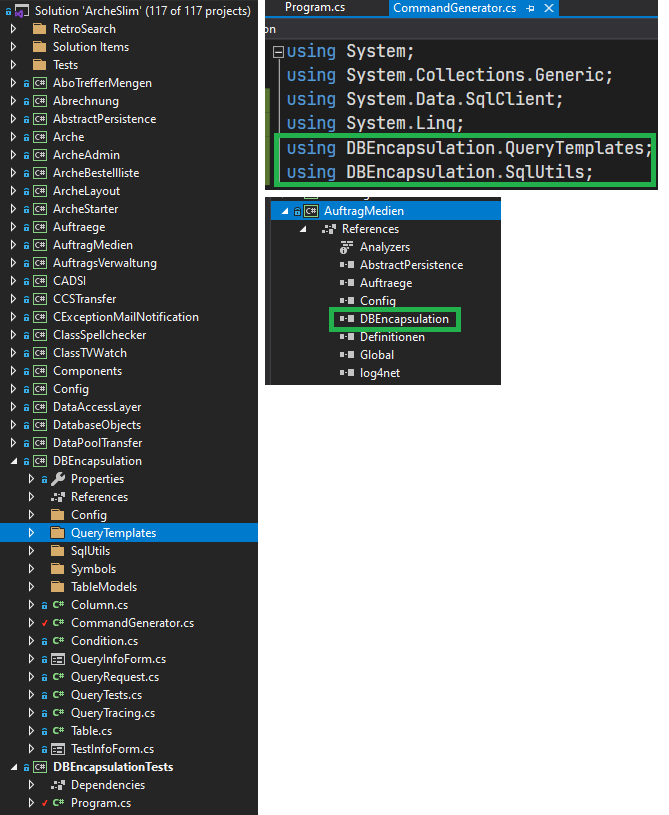
\includegraphics[scale=0.7]{Assemblies.png}
	 \caption{Assemblies und Referenzierung}
 \end{figure}
 \clearpage
 

 
 
 \subsection{Vermischung verschiedener Aufgabenbereiche}
 \label{fig:Vermischung verschiedener Aufgabenbereiche}
Anfang der Speichern-Funktion aus bereits vorhandenen GUI-Klasse. Diese erstreckt sich über mehrere Bildschirmseiten und vermischt Front- und Backend-Logik:
 \begin{figure}[htp]
 \centering

	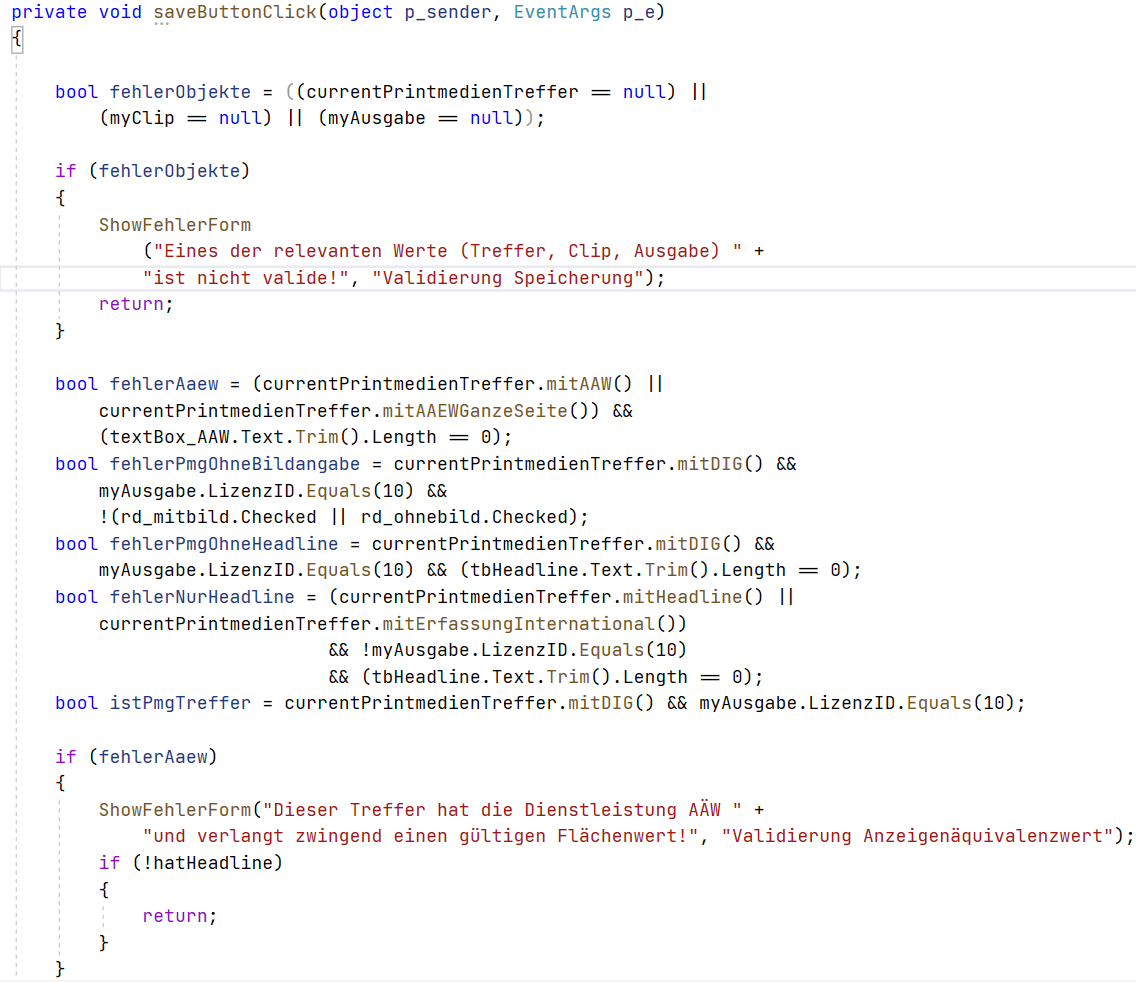
\includegraphics[scale=0.6]{SeparationOfConcerns.png}
	 \caption{Vermischung verschiedener Aufgabenbereiche}
 \end{figure}
 \clearpage

 \subsection{Auszug PrintmedienTreffer.cs}
 \label{fig:PrintmedienTreffer.cs}
Mehrere Variablen aus der bereits vorhandenen PrintmedienTreffer-Klasse. Manche sind noch in Benutzung, andere sind obsolet:
 \begin{figure}[htp]
 \centering

	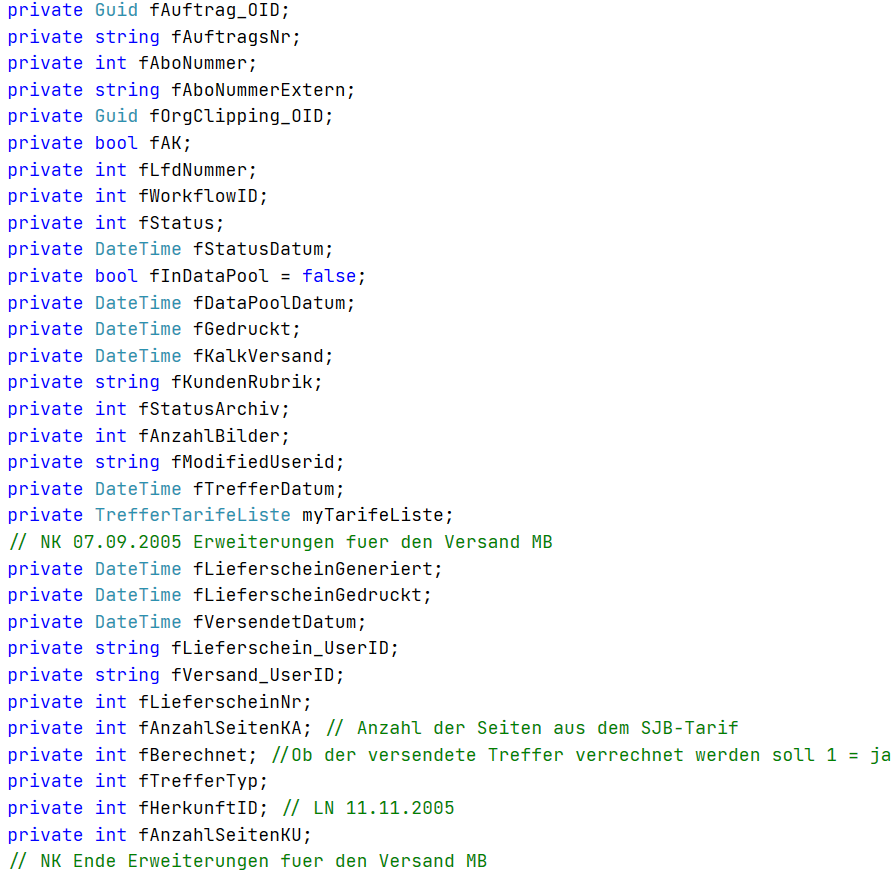
\includegraphics[scale=0.7]{PrintmedienTreffer.png}
	 \caption{PrintmedienTreffer-Auszug}
 \end{figure}
 \clearpage
 
  \subsection{Auszug AbstractTreffer.cs}
 \label{fig:AbstractTreffer.cs}
Mehrere Variablen aus der bereits vorhandenen PrintmedienTreffer-Klasse. Manche sind noch in Benutzung, andere sind obsolet:
 \begin{figure}[htp]
 \centering

	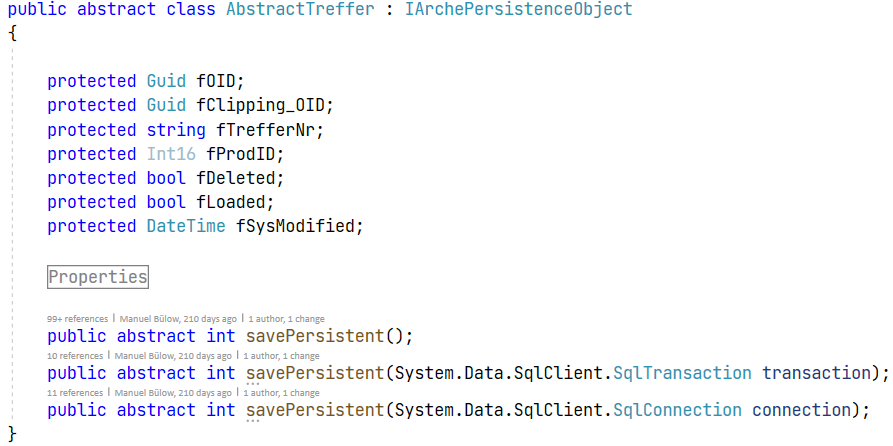
\includegraphics[scale=0.7]{abstractTreffer.png}
	 \caption{AbstractTreffer.cs}
 \end{figure}
 \clearpage
 
\subsection{Projektkosten Details}
	\label{sec:Projektkosten Details}
\begin{center}
\begin{table}[ht]

	%\hline\hline
		\begin{tabular}{|| p{27mm} | p{23mm} | r | r | r | r | r ||}
	    \hline	
	    
		\multicolumn{1}{||l|}{\textbf{Angefallen bei}}    &   \multicolumn{1}{|l|}{\textbf{Angefallen für}}  &   \multicolumn{1}{|c|}{\textbf{Std.}}  &  \multicolumn{1}{|c|}{\textbf{Lohn/Std.}}   & \multicolumn{1}{|c|}{\textbf{Lohn}} & \multicolumn{1}{|c|}{\textbf{Zschlg. 30\%}}    &   \multicolumn{1}{|c||}{\textbf{Summe}}   \\ 
		\hline
		
		
		Entwickler          & Fachliche\newline Unterstützung   &	4	& 40,00 €	& 160,00 €	    & 48,00 €	    & 208,00 €\\
		%\hline
		Ausbilder           &	Einarbeitung\newline Betreuung  &	8	& 45,00 €	& 360,00 €	    & 108,00 €	    & 468,00 €\\
		%\hline
		Praktikant          &	Durchführung \newline Projekt   &	70	& 10,00 €	& 700,00 €	    & 210,00 €	    & 910,00 €\\
		%\hline
		PO      &	Bereitstellung\newline Kosteninfo           &	2	& 60,00 €	& 120,00 €	    & 36,00 €	    & 156,00 €\\
		\hline%\hline
		Personal            &	                                &	84	& 155,00 €	& 1.340,00 €    & 402,00 €	    & 1.742,00 €\\
		\hline
		\multicolumn{6}{||l|}{Notebook für die Dokumentation}                                                       & 72,00 €\\
		\multicolumn{6}{||l|}{Desktop-PC für die Entwicklung}                                                       & 69,00 €\\
		\multicolumn{6}{||l|}{Infrastruktur Hardware (Netzwerk, VPN, Server, Verkabelung)}                          & 170,00 €\\
		\multicolumn{6}{||l|}{Peripheriegeräte (Docking Station, Maus, Tastatur, Headset)}                          & 190,00 €\\
		\multicolumn{6}{||l|}{Infrastruktur Software (Scrum-Tools, Windowslizenz)}                                  & 60,00 €\\
		\multicolumn{6}{||l|}{Visual Studio Professional Lizenz}                                                    & 140,00 €\\
		\hline
		\multicolumn{6}{||l|}{Technik}                                                                              & 701,00 €\\
		\hline
		\multicolumn{6}{||l|}{\textbf{Gesamt}}                                                                      &\textbf{2.443,00 €}\\
		\hline
		
			\end{tabular}
			\caption{Projektkosten Details}
			\end{table}
			\end{center}
			
				
			
	
	
		
		
		%\clearpage

\subsection{Zeitersparnis}
	\label{sec:Zeitersparnis}
%\begin{center}
\begin{table}[ht]
\centering
	%\hline\hline
		\begin{tabular}{|| l | r | r | r | r ||}
	    \hline
	    
		\textbf{Arbeitsschritt}                                     & \textbf{Mntl.} &\textbf{vorher} & \textbf{nachher} &\textbf{Gespart}\\
		\hline
		Identifizierung von Queries (Debug)                         & 36        & 10 min         & 2 min	         & 288 min\\
		Übertragen von Spaltennamen von SSMS nach VS2019            & 2         & 20 min         & 0 min	         & 40 min\\
		Verfassen der Insert-, Update- und Delete-Query             & 6         & 10 min         & 0 min	         & 60 min\\
		Manuelles Übertragen der Datentypen von SQL nach .NET       & 6         & 10 min         & 0 min	         & 60 min\\
		Hinzufügen der SQL-Parameter zu SQL-Command                 & 6         & 15 min         & 0 min	         & 90 min\\
		Prüfung der Daten durch Mitarbeiter                         & 6         & 40 min         & 0 min	         & 240 min\\
		\hline		
		\multicolumn{4}{||l|}{\textbf{Gesamtersparnis pro Monat}}                                                &\textbf{778 min}\\
		\hline
		
		
			\end{tabular}
			\caption{Zeitersparnis}
			\end{table}
			%\end{center}
			

\clearpage
\subsection{Anwendungsfalldiagramm}
In diesem Diagramm wird \glqq Query Tracer\grqq{} wie eine Person oder Firma behandelt. Dies ist insofern sinnvoll als dass die Entwicklerin nicht mit Argus, sondern mit firmeneigener Software interagiert. \glqq Lokale Datenbank erstellen\grqq{} könnte auch von \glqq Query Tracing aktivieren\grqq{} abhängen, ist andererseits aber auch ein eigenständiger Arbeitsschritt.
 \label{fig:Anwendungsfalldiagramm}

 \begin{figure}[htp]
 %\centering

	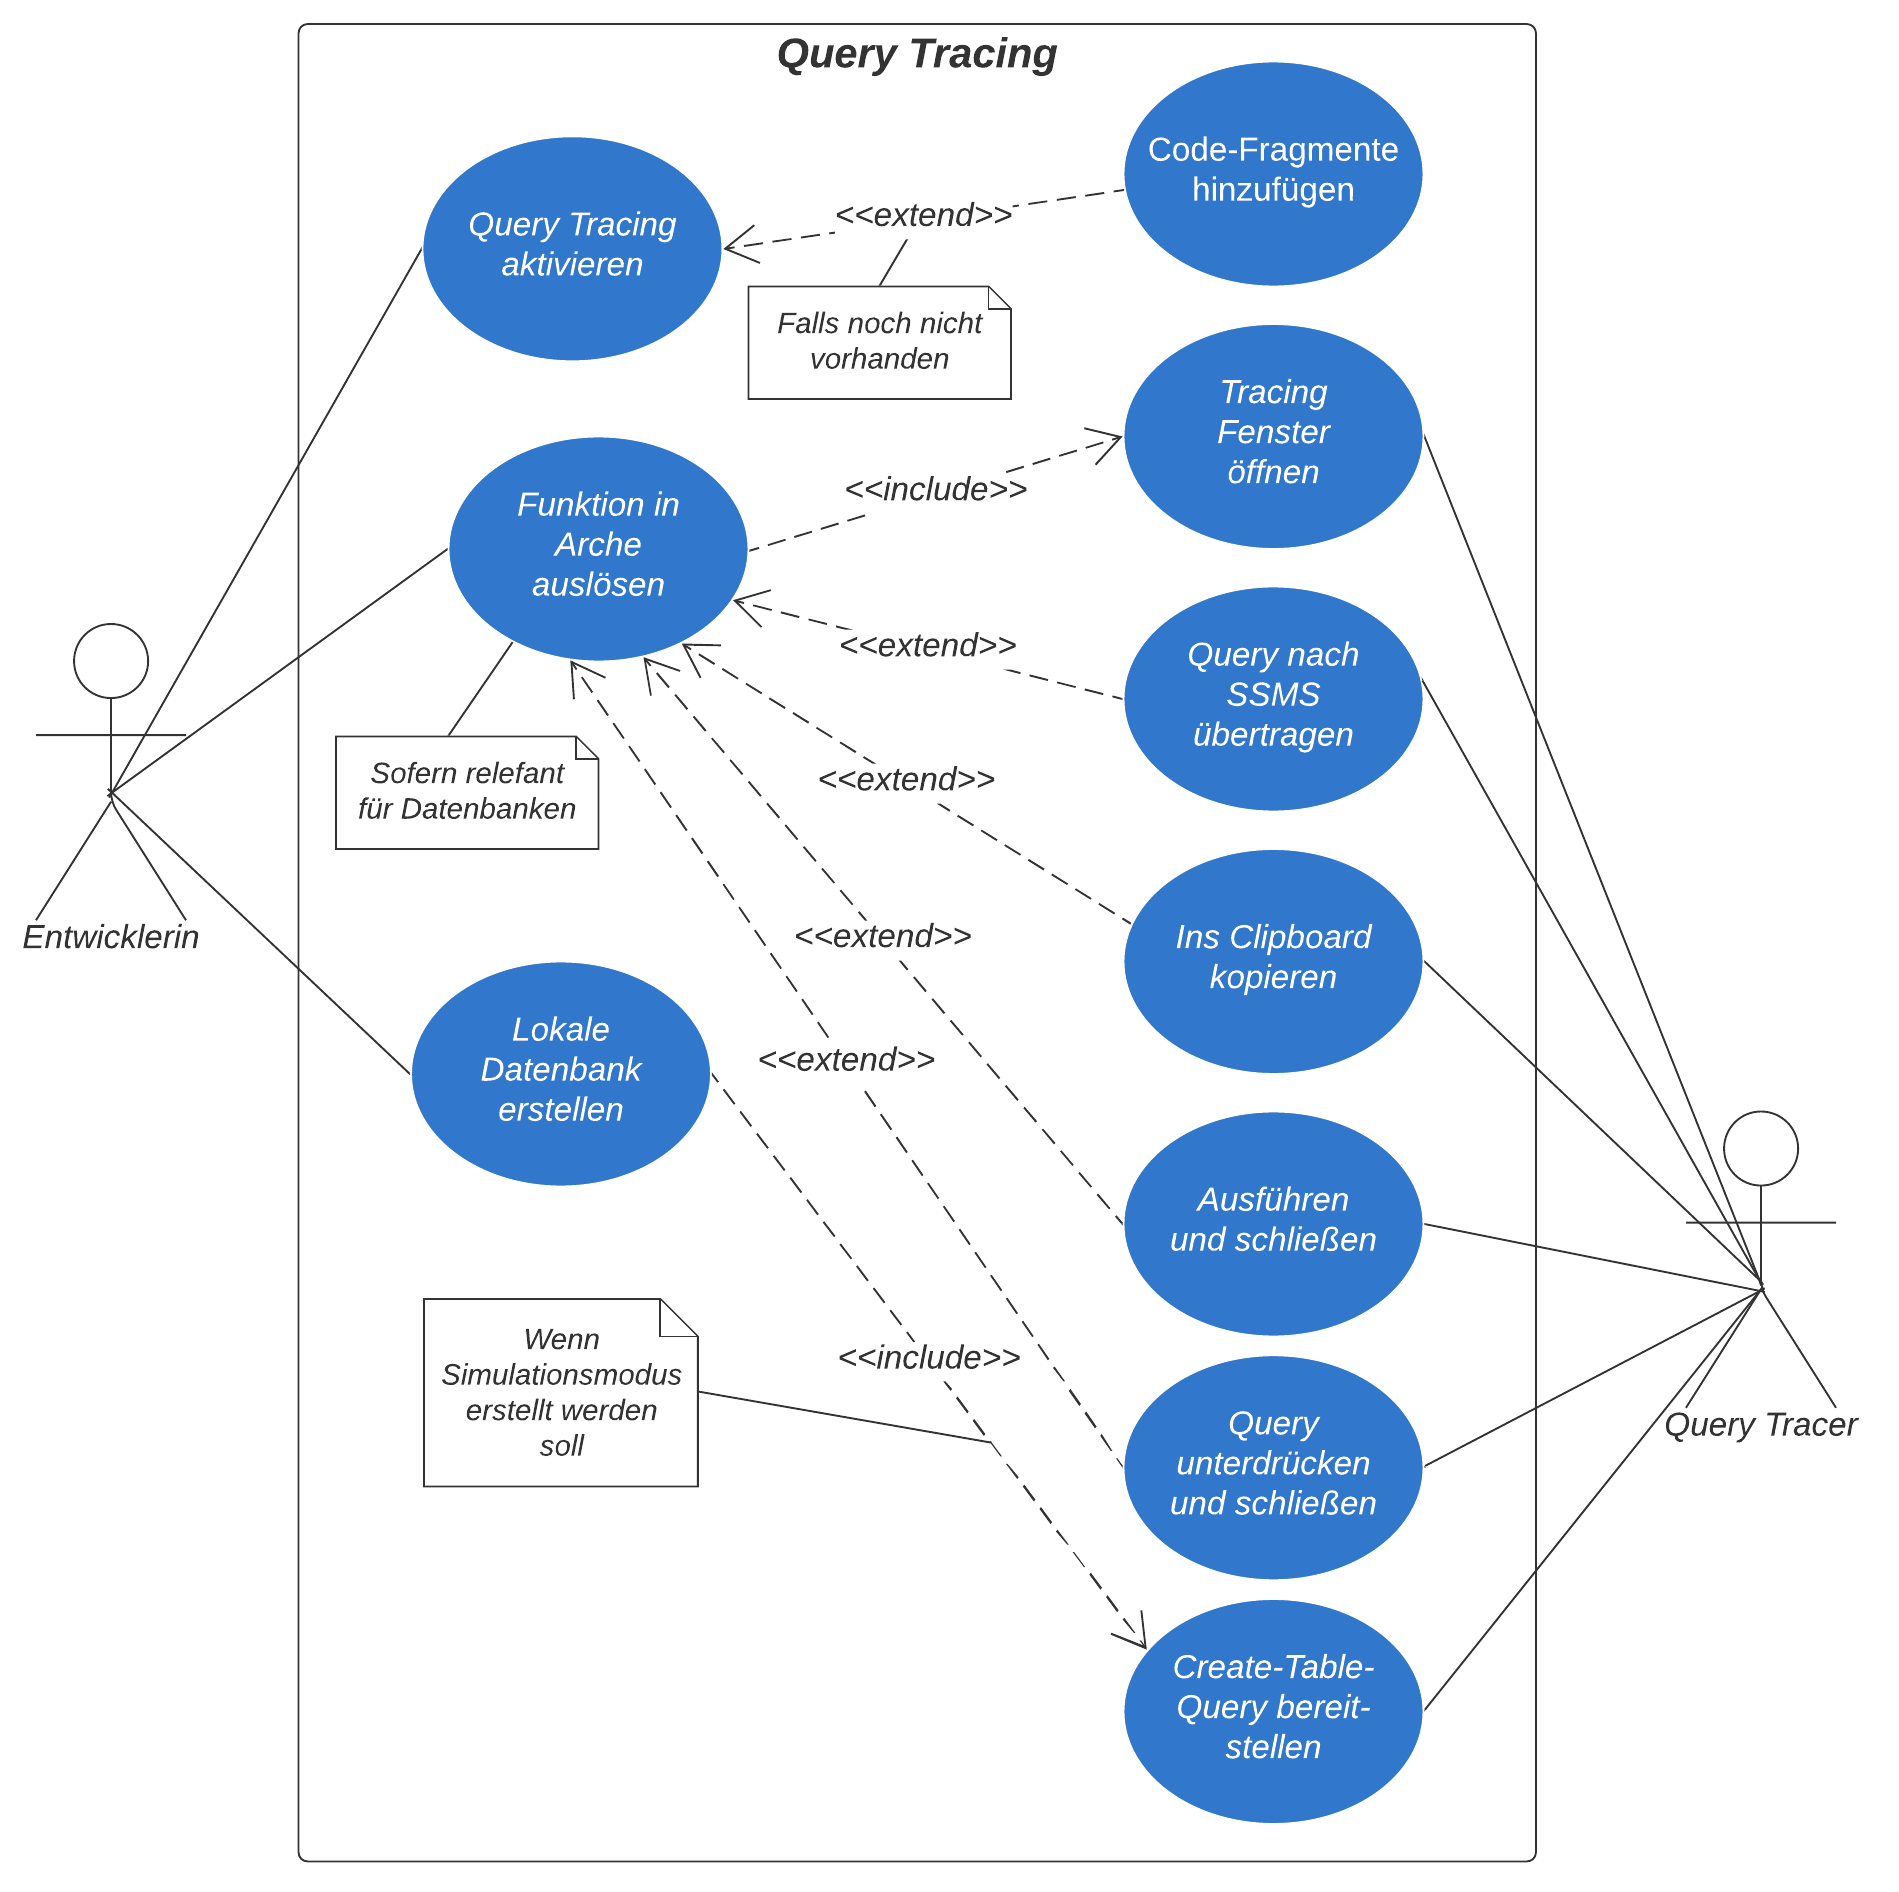
\includegraphics[scale=1.1]{Anwendungsfalldiagramm.png}
	 \caption{Anwendungsfalldiagramm}
 \end{figure}
 \clearpage
 

\subsection{Lastenheft (Auszug)}
\blindtext\blindtext

\subsection{Quell- und Zieldatenschema}
\blindtext\blindtext

\subsection{Sequenzdiagramm}
\blindtext


\subsection{Klassendiagramm}

Dies ist ein Beispiel für ein UML-Klassendiagramm:\\

\begin{comment}
 \begin{figure}[ht]
 \centering
 \begin{tikzpicture}

 	\umlclass[x=5, y= 0]{Person}	
 		{
 			- vorerkrankungen : String\\
 			- religion : string\\
 			+ alter : int\\
 			+ name : String\\
 			+ geschlecht : String\\
			
 		}
 		{
 			+ halloSagen() : void		\\	
 			+ freundlichLaecheln() : void		\\	
 		}
		
		
 	\umlclass[x=0, y= -6]{Kind}	
 		{
 			- kinderGarten: String\\
 			+ hobbys : String \\
 			+ magNutella : bool \\
 		}
 		{
 			- inDieSchuleGehen() : void	\\
 			- dreiradFahren() : void\\
 			+ getKindergarten() : String\\
			
 		}	
		
		
 	\umlclass[x=10, y= -6]{Erwachsener}	
 		{
 			- beruf: String\\
 			- kontostand : double\\
 			+ hatKinder : bool\\
 		}
 		{
 			- zurArbeitGehen() : void	\\
 			- autoFahren() : void\\
 			+ getBeruf() : String\\
			
 		}
		
 		\umlnote{Person}{Dies ist offensichtlich eine Klasse}		
 		\umlinherit[geometry=|-]{Erwachsener}{Person}
 		\umlinherit[geometry=-|]{Kind}{Person}
 		\umldep[very thick, arg1=0..*, arg2=1..*, pos1=0.05, pos2=0.52,anchor1=-20, anchor2=-20]{Kind}{Erwachsener}

	
 \end{tikzpicture}

 \caption{Klassendiagramm}
 \label{fig:Klassendiagramm}
	
 \end{figure}

\end{comment}

\subsection{Pflichtenheft (Auszug)}
Dies ist ein bisschen Text

\subsection{Laufzeitdiagnose}
\blindtext

\subsection{Ganttdiagramm}
\blindtext

\subsection{Projektstrukturplan}
\blindtext

\subsection{Arbeitspakete}
\blindtext

\subsection{Arbeitspaketressourcen im Detail}
\blindtext

\end{document}